\section{General problem}

Given the ARMAX system:
\[\mathcal{S}:y(t)=\dfrac{B(z)}{A(z)}u(t-k)+\dfrac{C(z)}{A(z)}e(t) \qquad e(t)\sim WN(0,\lambda^2)\]
We have the following assumptions:
\begin{itemize}
    \item $b_0\neq 0$. 
    \item $B(z)$ has all the roots strictly inside the unit circle.
    \item $\frac{C(z)}{A(z)}$ is in canonical representation. 
    \item $y^{0}(t)\perp e(t)$. 
    \item $y^{0}(t)$ is unpredictable, so $\hat{y}^\circ(t+k|t)=y^{0}(t)$. 
\end{itemize}
Our goal is to minimize:
\[\min{J}=\mathbb{E}\left[\left(y(t)-y^{0}(t)\right)^2\right]\]

\paragraph*{Optimality condition}
The primary method to solve this problem is to split $y(t)$  into predictor and error. 
Remembering that the prediction error is defined as $\varepsilon(t)=y(t)-\hat{y}(t\mid t-k)$, we have:
\[y(t)=\hat{y}(t\mid t-k)+\varepsilon(t)\]
We can now compute the performance index as:
\begin{align*}
    J   &=\mathbb{E}\left[\left(\hat{y}(t\mid t-k)+\varepsilon(t)-y^{0}(t)\right)^2\right] \\
        &=\mathbb{E}\left[\left(\left(\hat{y}(t\mid t-k)-y^{0}(t)\right)+\varepsilon(t)\right)^2\right] \\
        &=\mathbb{E}\left[\left(\hat{y}(t\mid t-k)-y^{0}(t)\right)^2\right]+\underbrace{\mathbb{E}\left[\varepsilon(t)^2\right]}_{\text{not }u(t)\text{-dependent}} +2\underbrace{\mathbb{E}\left[\left(\hat{y}(t\mid t-k)-y^{0}(t)\right)\varepsilon(t)\right]}_0 
\end{align*}
As a result, minimizing $J$ with respect to $u(t)$  is equivalent to minimizing the expected value of:
\[\min\mathbb{E}\left[\left(\hat{y}(t\mid t-k)-y^{0}(t)\right)^2\right]\]
This is minimum when:
\[\hat{y}(t\mid t-k)=y^{0}(t)\]
That is the optimality equation.

\paragraph*{Optimal predictor}
To find the optimal predictor, we perform $k$ steps of the long division between $C(z)$ and $A(z)$, obtaining a quotient $E(z)$ and the residual $R(z)=\tilde{R}(z)z^{-k}$. 
Thus, we have:
\[\dfrac{C(z)}{A(z)}=E(z)+\dfrac{\tilde{R}(z)z^{-k}}{A(z)}\]
The optimal predictor of an ARMAX system is then given by:
\[\hat{y}(t+k\mid t)=\dfrac{B(z)E(z)}{C(z)}u(t-k)+\dfrac{\tilde{R}(z)}{C(z)}y(t)\]
To ensure the optimality condition $\hat{y}(t+k\mid t)=y^{0}(t+k)$, we impose that $\hat{y}(t+k\mid t)=y^{0}(t)$: 
\[y^{0}(t)=\dfrac{B(z)E(z)}{C(z)}u(t-k)+\dfrac{\tilde{R}(z)}{C(z)}y(t)\]
We can now isolate $u(t)$ to find the controller algorithm: 
\[u(t)=\dfrac{1}{B(z)E(z)}\left(C(z)y^{0}(t)-\tilde{R}(z)y(t)\right)\]
This formula represents the general Minimum Variance Control controller.
\begin{figure}[H]
    \centering
    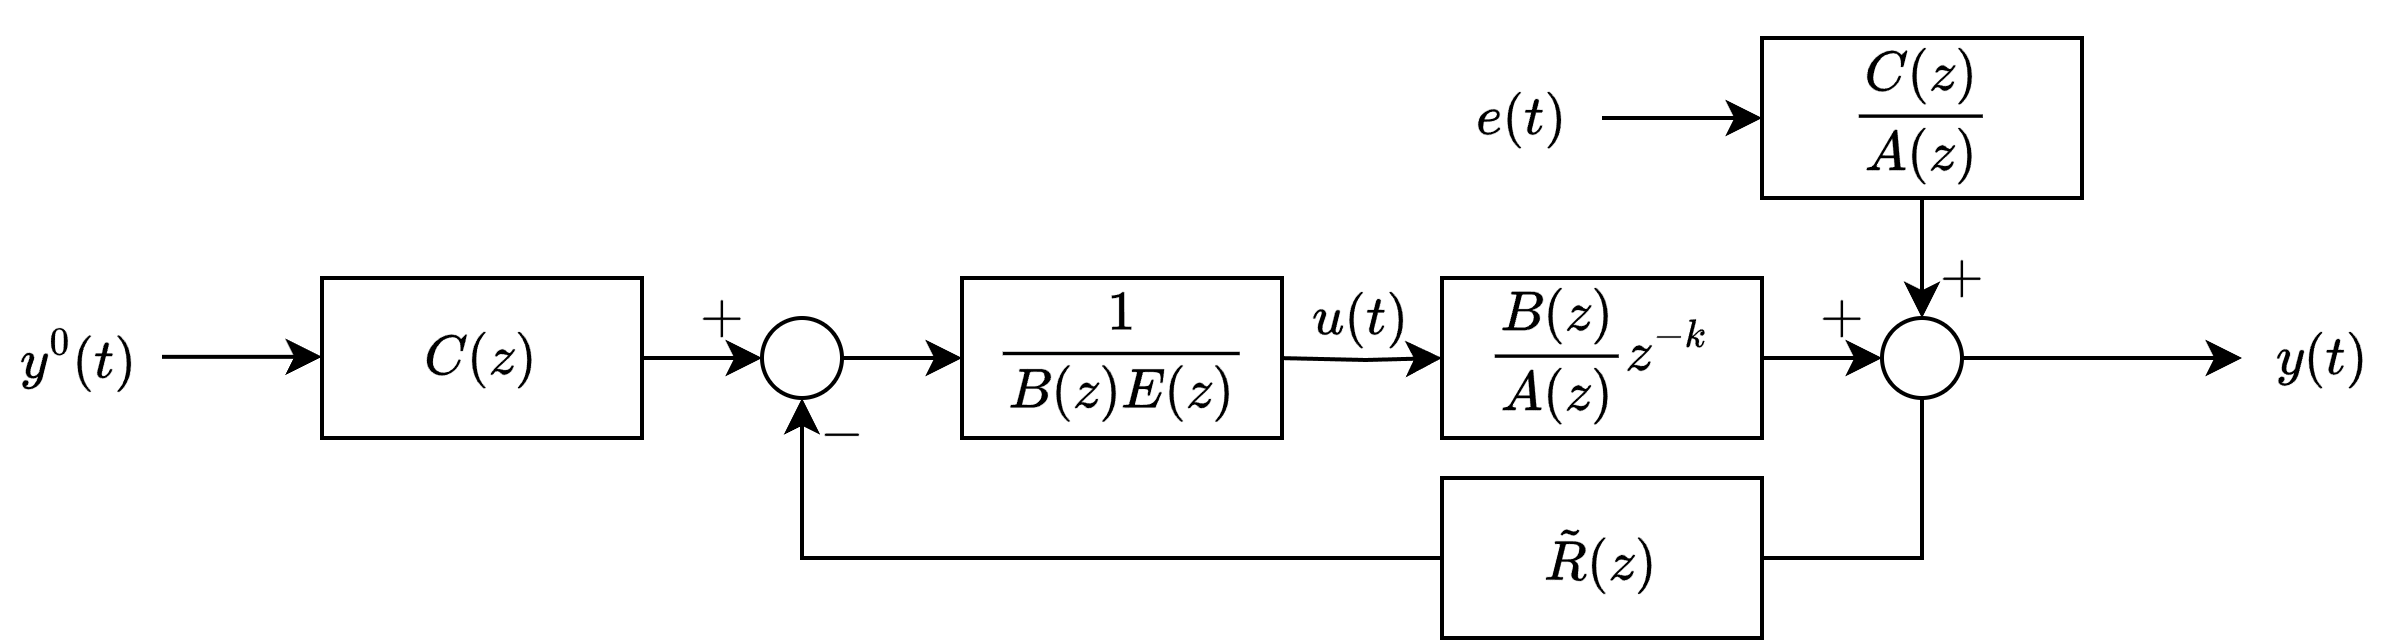
\includegraphics[width=0.75\linewidth]{images/fcss.png}
    \caption{Full control system scheme}
\end{figure}